\documentclass[12pt, a4paper, openany, twoside]{book}
\usepackage[italian]{babel}
\usepackage[T1]{fontenc}
\usepackage[utf8]{inputenc}
\usepackage{amsmath} 
\usepackage{xcolor}
\usepackage[margin=1in]{geometry}
\usepackage{hyperref}
\usepackage{graphicx}
\usepackage{listings}
\graphicspath{{./img/}}
\usepackage{tikz}
\hypersetup{
colorlinks=true,
linkcolor=blue,
filecolor=magenta,      
urlcolor=cyan,
}

\begin{document}
\fontfamily{cmss}\selectfont
\pagestyle{plain}
\author{DaveRhapsody}
\title {Laboratorio di Linguaggi e Computabilità}
\date {30 Ottobre 2019}
\maketitle
\tableofcontents
\chapter{LeX \& Yacc}
Sono due software complementari atti a sviluppare dei compilatori. Più precisamente
sono un \textbf{Parser} ed un \textbf{Lexer}
\section{parser}
Un parser semplicemente analizza quella che è la grammatica formale (quello che
vi dice se è giusto il codice che avete scritto). 
\begin{itemize}
	\item Produce un albero sintattico
	\item Ha bisogno di considerare il testo tramite dei Token (vedremo in seguito
	da dove arrivano)
	\item Ricorre all'analizzatore lessicale (Lexer, quello che analizza la 
	sequenza di carattere)
\end{itemize}
Essendo due programmi distinti, sono sviluppabili entrambi. Per dire il parser
lo possiamo sviluppare con C o C+.
In questo caso sfrutteremo dei tool fatti apposta per generare sia il parser che
il Lexer.
\paragraph{Come funziona?}
Il Lexer analizza carattere per carattere, e non fa altro che sparare al parser
dei token che verranno analizzati. Più precisamente il lexer produce \textbf{
grammatiche regolari
} mentre il parser produce \textbf{grammatiche context-free} 
\paragraph{Altra cosa formale: }
Noi si lavorerà con i generatori, per fare in modo di avere Parser e Lexer, perchè
di fatto quello che accade è che si genera un automa a pila.
\begin{enumerate}
	\item Gli si dà un file al generatore di parser
	\begin{itemize}
		\item Quello che faremo sarà ragionare su questi file, la parte più 
		rognosa è questa alla fine.
		\item Composto da tre sezioni, ma le vedremo in seguito.
		\item Spoiler:
		\begin{enumerate}
			\item Dichiarazioni
			\item Regole di traduzione
			\item Procedure ausiliarie
		\end{enumerate}
	\end{itemize}
	\item Il generatore di parser mi genera il codice sorgente del parser
\end{enumerate}
\section{Generatore di Lexer}
Come detto sopra il lexer è una specie di scanner, ed il file di input che va 
al lexer sarà un pattern. Ogni pattern avrà a sè associata una action, ossia
un frammento di programma che ti dà un token. 
\paragraph{Cos'è un token? }Molto semplicemenente è una stringa che viene 
riconosciuta da un pattern.
Invece Lex va a generare un programma che implementa un automa a stati finiti
\section{La struttura di un file}
Stessa struttura dei file .y usati con le versioni di Yacc per generare codice
C/C++
\begin{center}
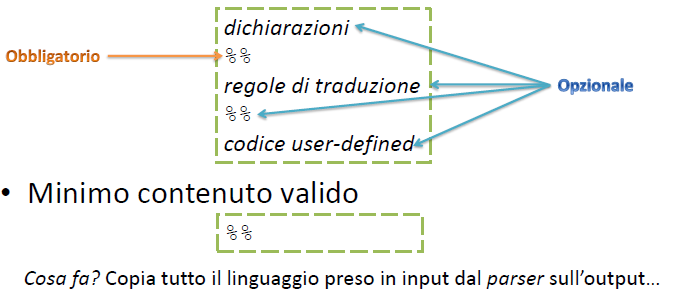
\includegraphics[width=0.75\textwidth]{1}
\end{center}
\section{Definizione della grammatica}
Definiamo il concetto di simbolo
Si divide in tre macrocategorie:
\subsection{Simboli non terminali}
Per convenzione vanno scritti in \textbf{minuscolo}, sono dei normali nomi ma
semplicemente
si scrivono in minuscolo
\paragraph{Esempio: }Non terminali: \%type nome Es.: \%type string\_ass
\subsection{Simboli terminali (token)}
Per convenzione questi invece vanno in \textbf{MAIUSCOLO}
\paragraph{Esempio: }Terminali: \%token NOME Es.: \%token NUM
\subsection{Regole sintattiche}
Sono le famose 'Produzioni' già affrontate a lezione.
Fondamentalmente questi simboli si definiscono nella sezione dichiarativa. 
\paragraph{Per default: }tutti i simboli sono di tipo int, ma è possibile
utilizzare altri tipi di dato
\begin{enumerate}
	\item La classe ParserVal fornisce dei metodi che permettono l’uso di tipi 
	di dato differenti da int
	\item Associando il tipo ai simboli terminali e non terminali attraverso
	l’uso di parentesi angolari nei costrutti che ne permettono la dichiarazione
\end{enumerate}
\section{Definizione delle regole}
\begin{center}
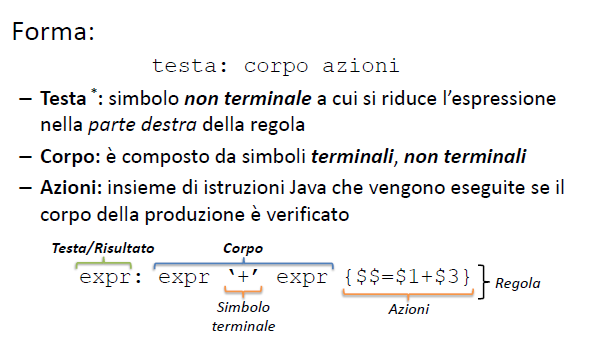
\includegraphics[width=0.75\textwidth]{2}
\end{center}
E' possibile elencare "parti destre" alternative che portano alla riscrittura
dello stesso simbolo \textit{Non terminale} nella parte sinistra
\begin{lstlisting}[language=Prolog]
expr: expr "+" expr {$$=$1+$3} |
expr "*" expr {$$=$1*$3};
\end{lstlisting}
Se la parte destra è vuota allora la produzione viene soddisfatta anche dalla
stringa vuota
\begin{lstlisting}[language=Prolog]
expr: /* stringa vuota */ |
expr_1;
\end{lstlisting}
La produzione è ricorsiva se il simbolo non terminale della parte sinistra
compare anche nella parte destra
\begin{lstlisting}[language=Prolog]
expr_seq: expr |
expr_seq "," expr;
\end{lstlisting}
\paragraph{Osservazione: }Dalle slides si consiglia di evitare un uso eccessivo
 della ricorsione, da Prolog tutto è ricorsivo, insomma qualcuno che si metta 
 d'accorod in questo corso è difficile a trovarsi. 
 \section{Produzioni ed azioni}
 \subsection{L'azione }
 E' una parte di codice in Java che viene eseguita quando la produzione viene
 applicata (Riduzione).
 Concettualmente il valore dell'n-esimo elemento della produzione corrisponde
 a \$n; \$\$, e rappresenta la parte sinistra.
 \paragraph{SE non si specificasse nulla si avrebbe: } \$\$=S1,
 inoltre il tipo associato a \$n è quello dell'elemento corrispondente
 \subparagraph{Mi spiego peggio: } Si può forzare qualsiasi altro tipo, come
 si faceva con il casting, per intenderci, e si fa usando \$*Magico tipo per i
 dati*n
 \section{Associatività e Precedenza}
 E' possibile definire l'associatività dei simboli (sia a sinistra che a
 destra) MA allo stesso modo si può anche definire la precedenza IN BASE al'ordine
 delle dichiarazioni.
 \paragraph{Disclaimer importante: }
 (Da qui in poi conviene guardare le slides riportate nella cartella 
 'Materiale utile' perchè mi son reso conto che (ennesimamente) non sto facendo
 altro che riformulare le frasi scritte lì. ERGO, forse converrà di più guardarsi
 solo gli esercizi)
  	     	
     
\end{document}	
